\chapter{Vorlesung}
\subsection{Einfache Union-Find-Datenstruktur}
\begin{tabular}{c|c|c|c|c|c|}
	    &$0$&$1$&$2$&        &$n-1$\\ \hline
	ref &$0$&$1$&$2$&$\ldots$&$n-1$\\ \hline
	size&$1$&$1$&$1$&$\ldots$&  $1$\\ \hline
	next&$-1$&$-1$&$-1$&$\ldots$&$-1$\\ \hline	
\end{tabular}
$n=|V|$\\

\begin{wrapfigure}{r}{0.5\textwidth}
	\vspace{200pt}
	\centering
	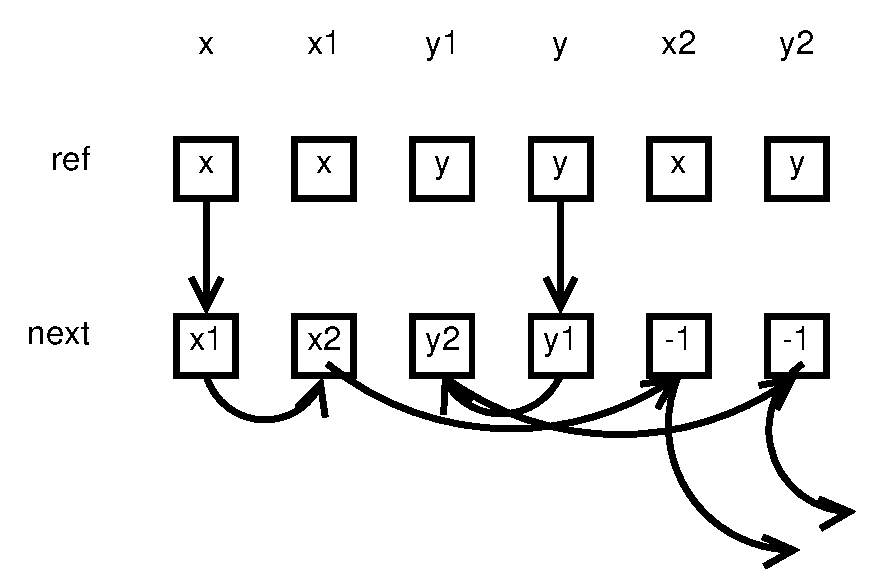
\includegraphics[width=\linewidth]{20/Grafik/img1}
\end{wrapfigure}
\begin{lstlisting}
class Partition
	int[] ref,size,next;
	Partiotion(int n) {
		ref = new int[n];
		size = new int[n];
		next = new int [n];
		for (int i = 0; i < n; i++) {
			ref[i] = i;
			size[i] = 1;
			next[i] = -1;
		}
	}
	int find(int v) {
		return ref[v];
	}
	void union(int u, int v) {
		int x = ref[u];
		int y = ref[v];
		
		if (size[x] > size[y]) {
			x = ref[v];
			y = ref[u];
		}
		int h = next[y];
		next[y] = x;
		int z = y;
		while( next[z] $\geq$ 0) {
			z = next[z];
			ref[z] = y;
		}
		next[z] = h;
		size[y] = size[y] + size[x];
	}
\end{lstlisting}
%Grafik1 eigentlich bei line 33

\subsubsection{Laufzeit Kruskal}
\[ \mathcal{O}(|E|\cdot\log|V|+|E|+|V|\cdot\log|V|) \]
\[ \mathcal{O}(|E|\cdot\log|V|) \]
\pagebreak
\subsection{Prim-Algorithmus zur Berechnung eines MST}

%Grafik 2 und 3
\begin{figure}[H]
\centering
\begin{subfigure}[h]{0.4\textwidth}
	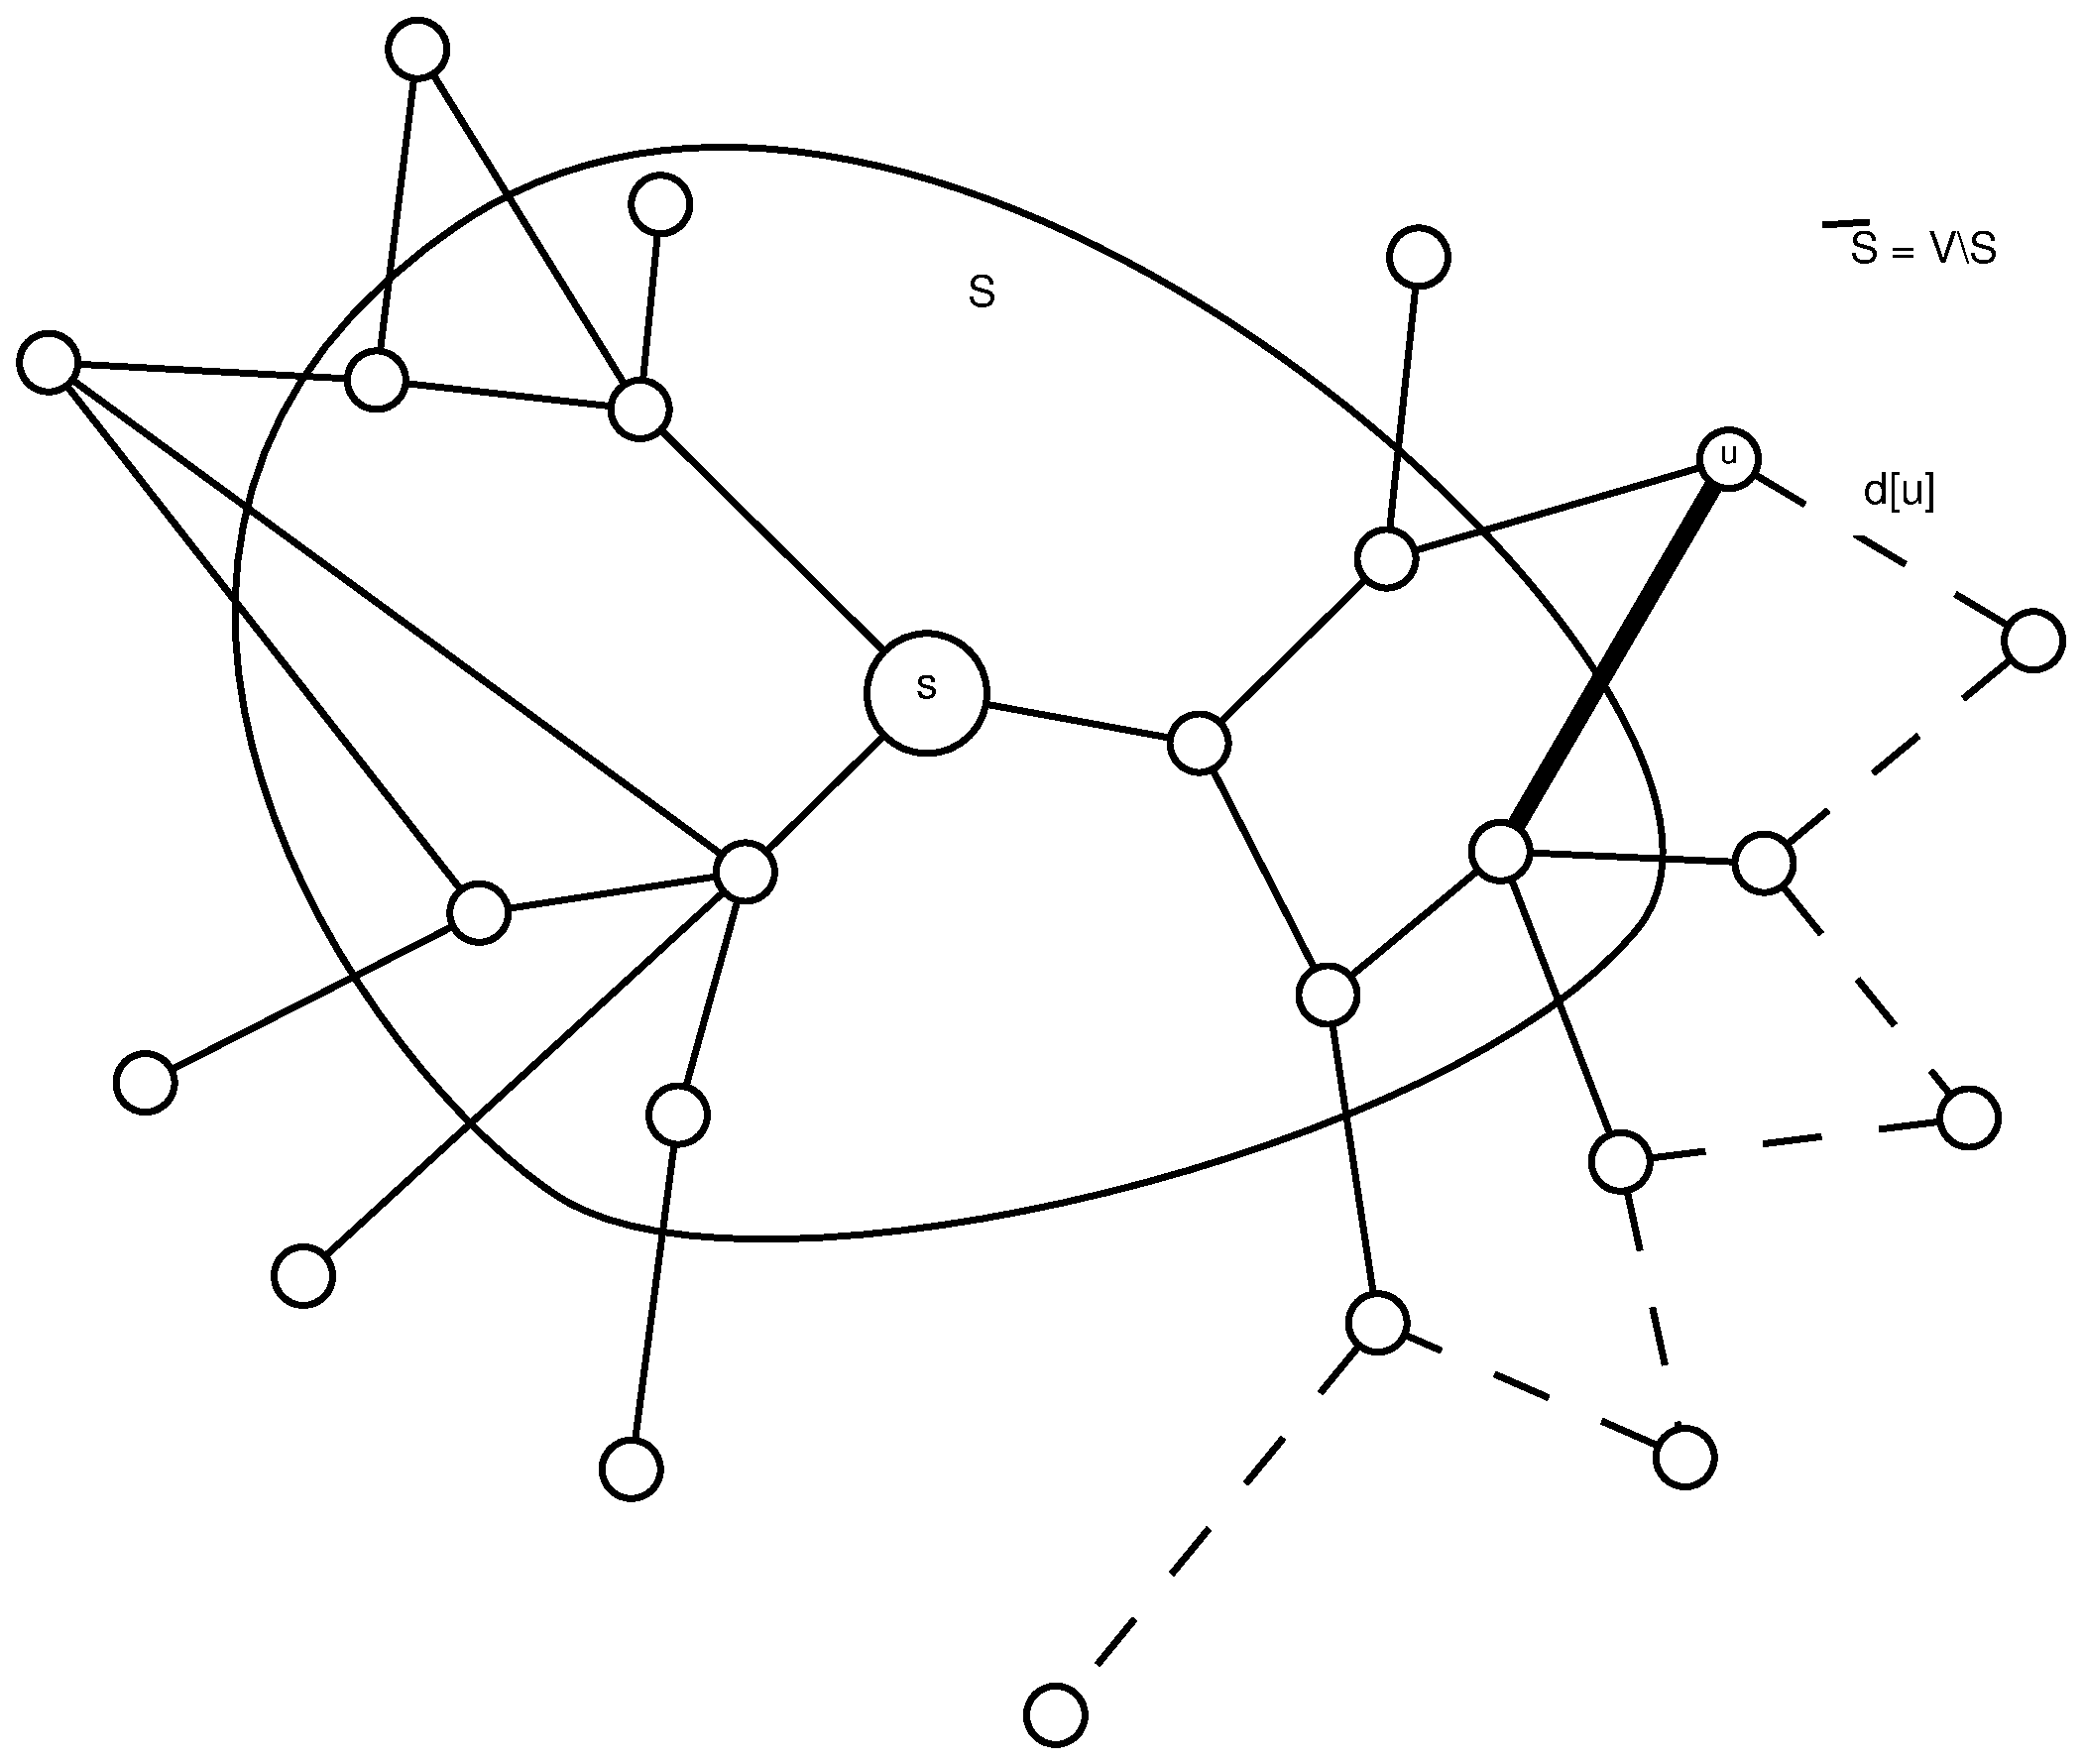
\includegraphics[width=\linewidth]{20/Grafik/img2}
	\[ \overline{S} = V \setminus S \]
\end{subfigure}
\begin{subfigure}[h]{0.4\textwidth}
	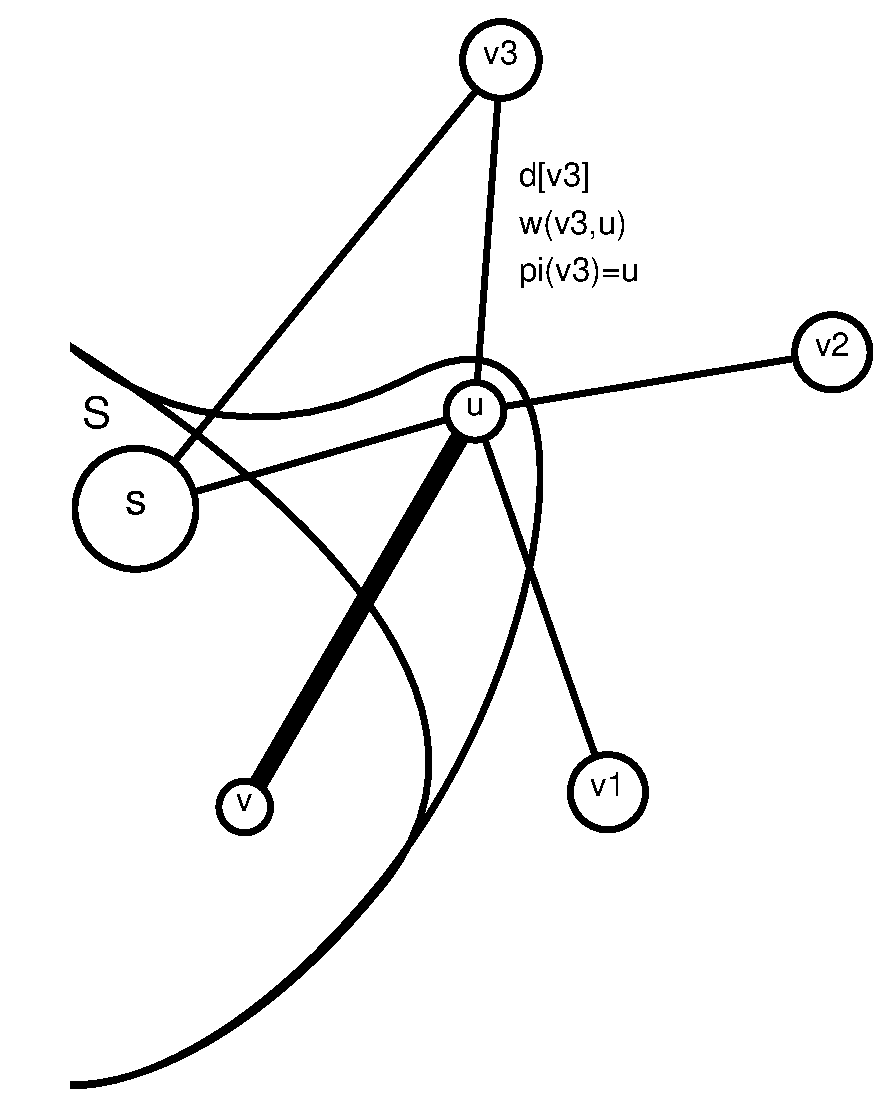
\includegraphics[width=\linewidth]{20/Grafik/img3}
	\[ T=T\cup \{ (u,v) \} \]
	\[ T_{MST}=\{ (v,\pi(v))~|~v\in V\setminus\{ s \} \]
\end{subfigure}
\end{figure}

\begin{lstlisting}
PriotityQueue PQ;
forall(v $\in$ V) {
	d[v] = $\infty$;
	$\pi$[v] = NULL;
	inTree[v] = false;
	PQ.insert(v, d[v]);
}
d[s] = 0;
PQ.decreaseKey(s,d[s]);		//$\overline{S}\hat{=}PQ$
T = $\emptyset$				//$S\hat{=}\{ v\in V |$inTree[v] = true$\}$
while(!PQ.empty()) {
	u = PQ.deleteMin();
	forall((u,v)$\in$E) {
		if(inTree[v] == true) continue;
		if(d[v] > w(u,v)) {
			d[v] = w(u,v);
			$\pi$[v] = u;
			PQ.derceaseKey(v, d[v]);
		}
	}
	inTree[u] = true;
	T = T $\cup$ (u,v);	//T = T $\cup$ {(u,$\pi$[u])} u $\neq$ s
}
\end{lstlisting}
\subsubsection{Korrektheit des Prim-Algorithmus}
Korrektheit von Prim folgt unmittelbar aus dem Schnitt-Lemma, denn der Algorithmus stellt sicher, dass stets eine Kante gewählt wird, die mit minimalem Gewicht über den Schnitt $(S,\overline{S})$ führt.
\subsubsection{Laufzeit des Prim-Algoritmus}
\begin{tabular}{ll}
	$|V|\times$\texttt{PQ.insert}&$\mathcal{O}(1)$\\
	$|V|\times$\texttt{PQ.empty}&$\mathcal{O}(1)$\\
	$|V|\times$\texttt{PQ.deleteMin}&$\mathcal{O}(\log|V|)$\\
	$|E|\times$\texttt{PQ.decreaseKey}&$\mathcal{O}(1)$
\end{tabular}
In Summe $\mathcal{O}(|E|+|V|\cdot\log|V|)$

\newpage
\subsection{Beispiel des Prim-Algorithmus:}
\begin{figure}[H]
	\centering
	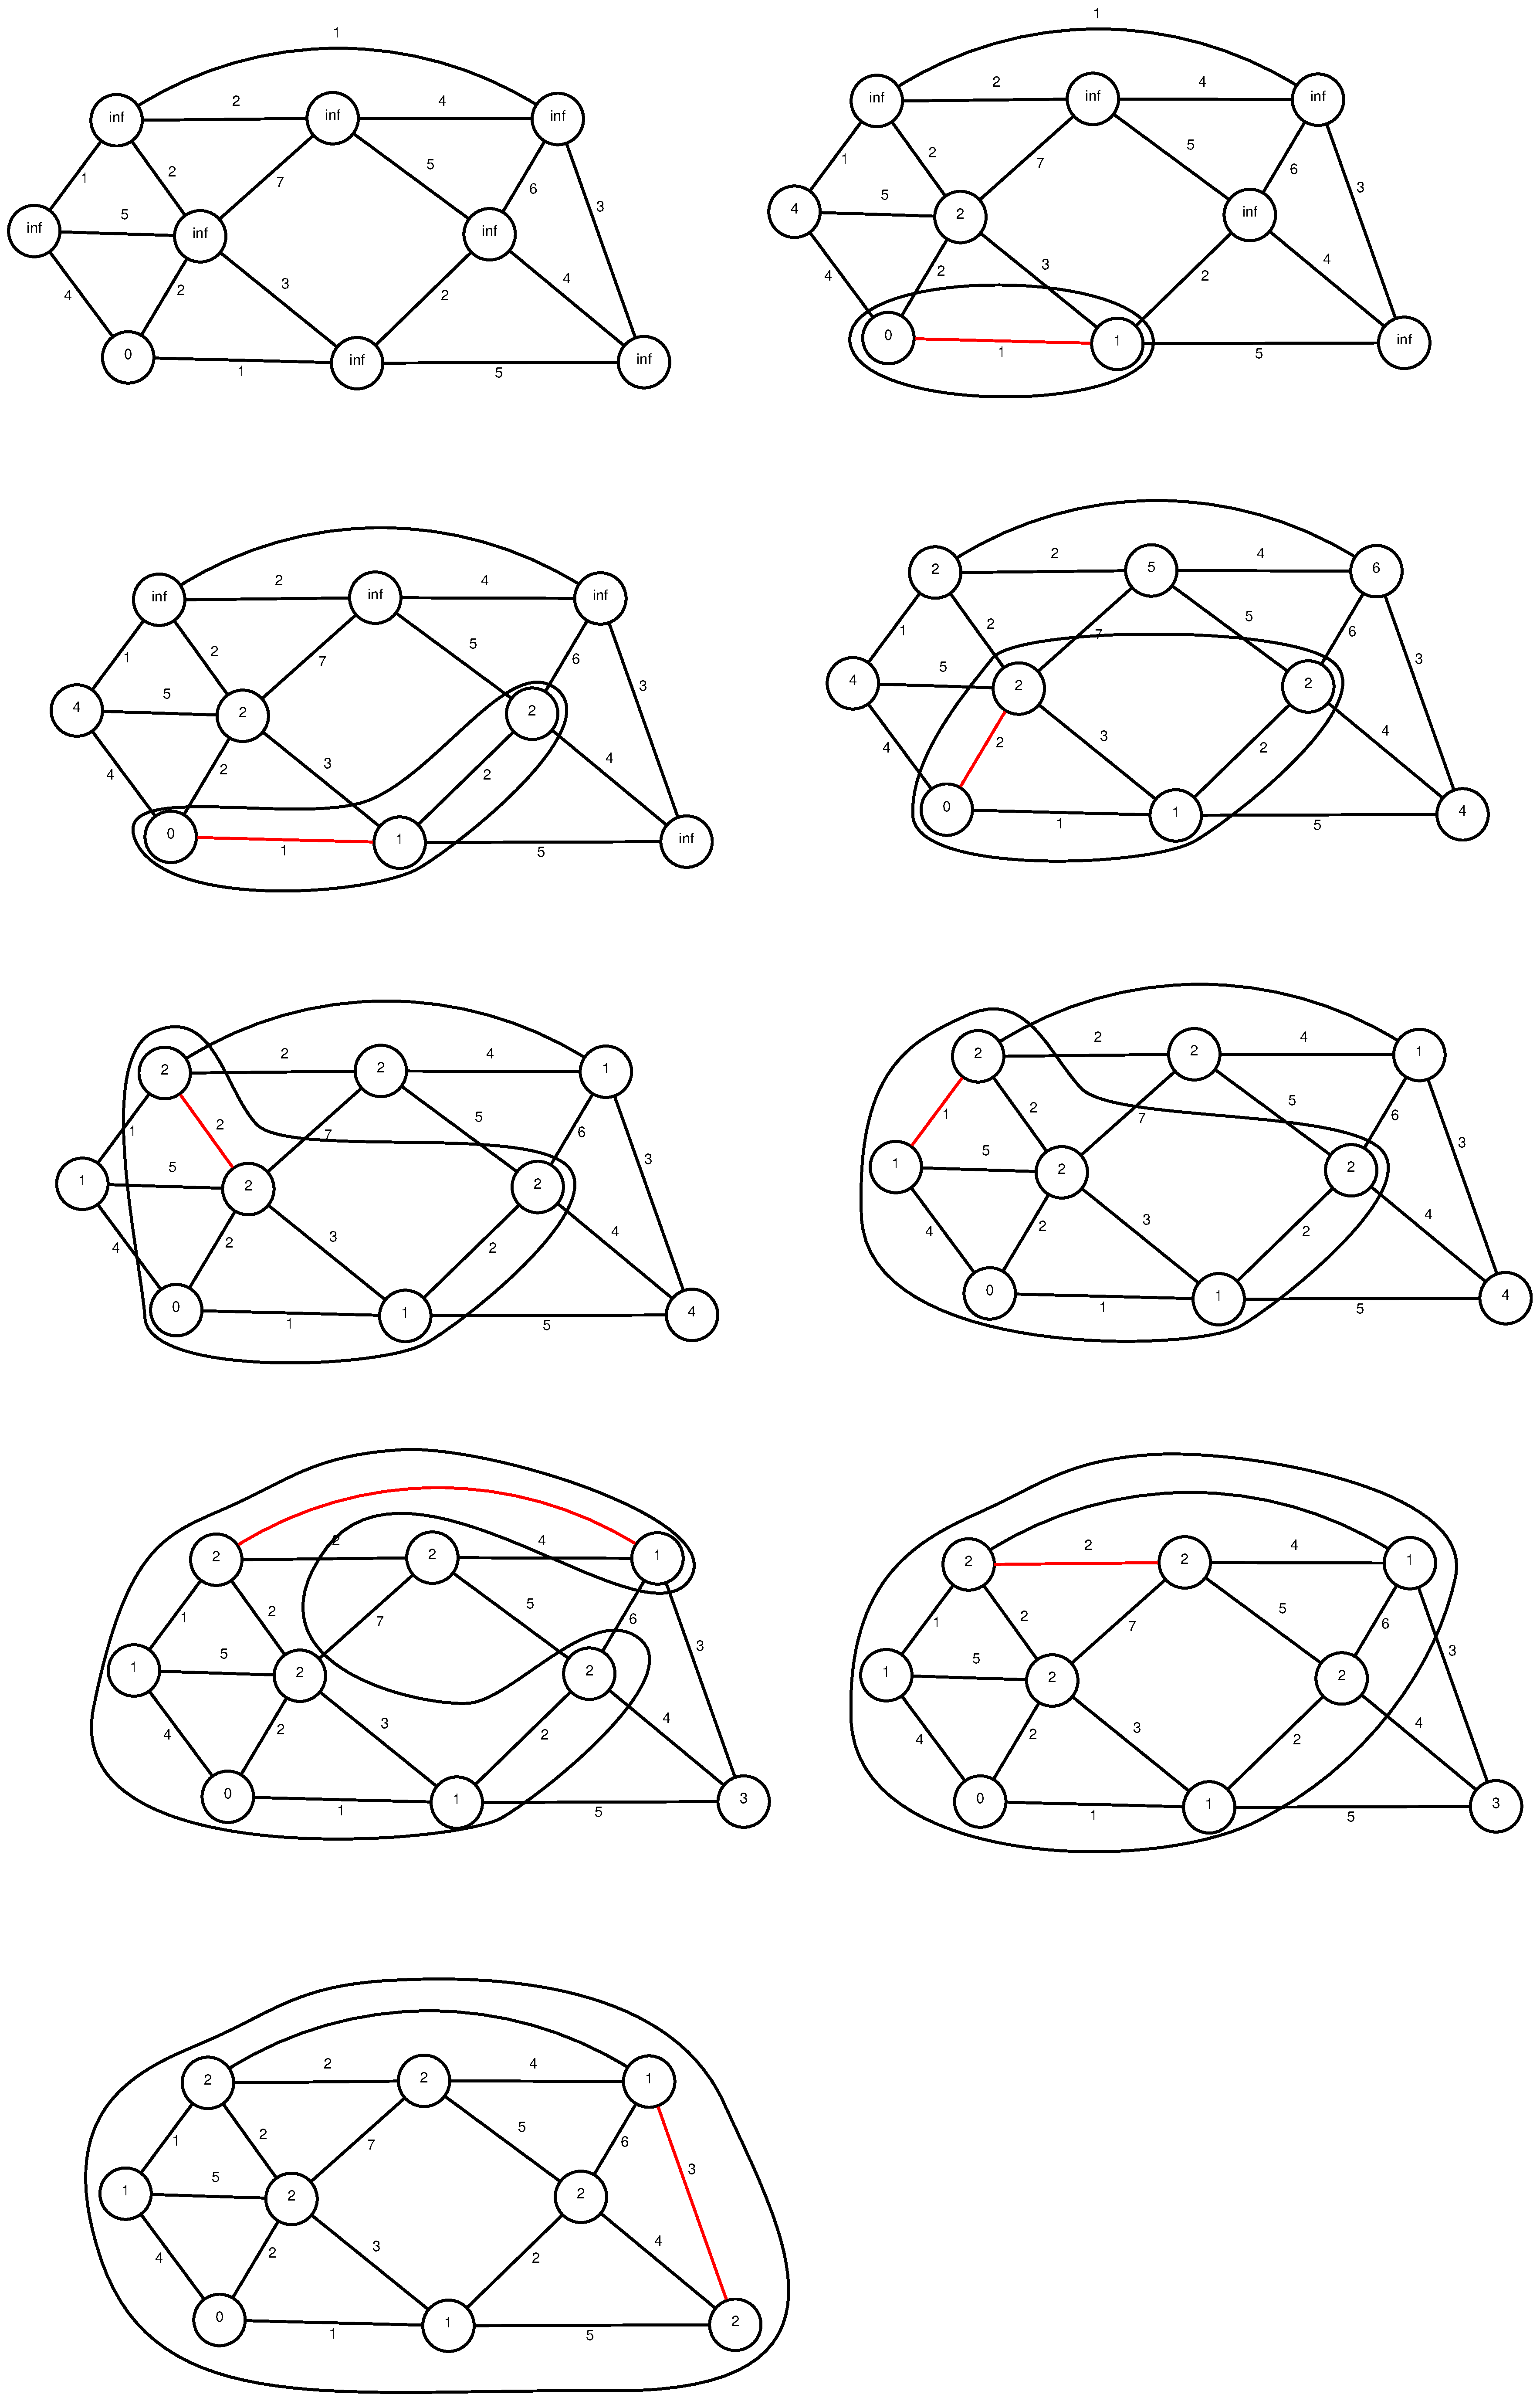
\includegraphics[width=0.65\linewidth]{20/Grafik/BspPrim}
	\caption{}
\end{figure}

